\chapter{Testare și validare}
\label{ch:testare}
\pagestyle{fancy}

După realizarea sistemului, atât pe partea hardware, cât și pe cea mecanică, a urmat
etapa de testare, prin care s-a verificat că fiecare componentă funcționează corect și
că ansamblul își îndeplinește scopul. Testarea a fost gândită pe niveluri, pornind de la
verificarea individuală a fiecărui element și avansând treptat către sistemul complet.
Această abordare, în care fiecare etapă se sprijină pe cea anterioară, permite
identificarea rapidă a eventualelor probleme, deoarece un element este integrat în
ansamblu abia după ce a fost validat separat. Succesiunea etapelor de testare este
prezentată în Figura~\ref{fig:etape-testare}.

\begin{figure}[H]
	\centering
	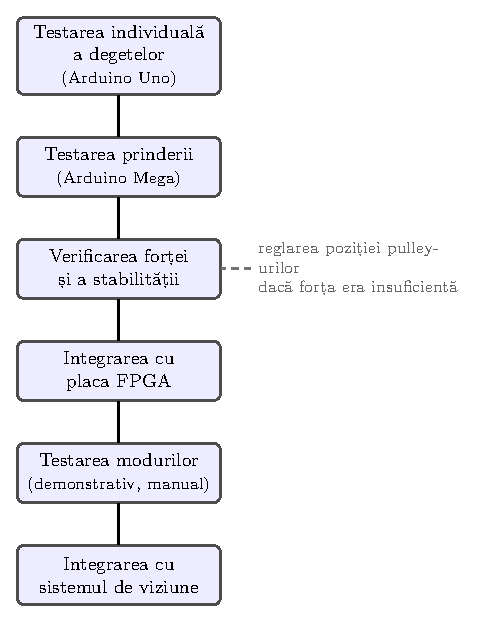
\includegraphics[width=0.5\textwidth]{figs/etape_testare.pdf}
	\caption{Succesiunea etapelor de testare, de la verificarea individuală a degetelor
	până la integrarea cu sistemul de viziune.}
	\label{fig:etape-testare}
\end{figure}

\section{Testarea individuală a degetelor}
\label{sec:testare-degete}

Primul pas a fost verificarea faptului că fiecare deget se mișcă corect, testat separat
înainte de a fi integrat în ansamblu. Pentru aceasta a fost folosită o placă Arduino Uno,
cu care s-a comandat pe rând câte un servomotor, urmărind dacă degetul corespunzător se
închide și se deschide complet, fără blocaje pe traseul firului. Această verificare
timpurie a permis depistarea din start a problemelor mecanice, precum firele prea strânse
sau canalele de ghidare cu frecare prea mare, care au putut fi corectate înainte de a
continua.

\section{Testarea și calibrarea servomotoarelor}
\label{sec:testare-servo}

După validarea individuală a degetelor, s-a trecut la testarea prinderii cu toate
servomotoarele acționate împreună, folosind o placă Arduino Mega, care dispune de
suficiente ieșiri pentru cele opt canale. Programul de test permite comanda fiecărui
servomotor printr-o interfață serială simplă, prin care un servomotor poate fi trimis la o
poziție anume sau se poate rula o secvență automată de baleiere pe întreaga cursă. Fiecare
servomotor are definite o poziție de pornire și limite proprii, iar cel corespunzător
mișcării palmare a degetului mare este limitat la un interval redus.

\begin{lstlisting}[language=C++,caption={Fragment din programul de test, comanda unui servomotor cu limitare la interval.},label={lst:arduino}]
void setServo(int idx, int a) {
    a = constrain(a, angleMin[idx], angleMax[idx]);
    angle[idx] = a;
    servos[idx].write(a);
}
\end{lstlisting}

Funcția de mai sus limitează unghiul cerut la intervalul admis pentru fiecare servomotor,
prin funcția \texttt{constrain}, după care comandă efectiv poziția. Această etapă de
testare a fost cea care a scos la iveală faptul că servomotoarele folosite nu parcurg
întreaga cursă la intervalul standard de 1 până la 2 milisecunde, oprindu-se mult înainte
de a atinge pozițiile extreme. Observația a condus la lărgirea intervalului PWM, până la
valorile care asigură cursa completă, atât în programul de test, cât și, ulterior, în
implementarea de pe placa FPGA.

\section{Verificarea forței și a stabilității}
\label{sec:testare-forta}

Un aspect esențial pentru o mână robotică funcțională este ca degetele să nu doar atingă
obiectul, ci să îl strângă cu o forță suficientă pentru a-l susține în mod stabil. Din
acest motiv, după validarea mișcării, s-a verificat forța de strângere a fiecărui deget.
Acolo unde forța s-a dovedit insuficientă, soluția a fost repoziționarea pulley-urilor pe
axul servomotorului, astfel încât firul să fie tras cu un braț de pârghie mai favorabil,
crescând forța de tragere. Prin astfel de ajustări succesive s-a obținut o strângere
fermă și uniformă pe toate degetele.

\section{Integrarea cu placa FPGA}
\label{sec:testare-integrare}

După validarea completă a părții mecanice, sistemul a fost conectat la placa Basys3, care
a preluat rolul de comandă în locul plăcii Arduino folosite pentru teste. Un rezultat
îmbucurător a fost acela că ansamblul a funcționat corect de la prima încercare, ceea ce
confirmă că etapele anterioare de testare și validare individuală și-au atins scopul,
reducând la minimum problemele de integrare. Această funcționare din prima reprezintă și o
dovadă a unei proiectări atente, în care fiecare subsistem a fost verificat înainte de a fi
adus în ansamblu.

Odată integrată placa, au fost testate pe rând cele două moduri autonome de funcționare.
Mai întâi modul demonstrativ, în care mâna parcurge o secvență predefinită de mișcări, a
confirmat că lanțul complet de prelucrare, de la generarea comenzilor până la actuarea
servomotoarelor, funcționează corect. Apoi a fost testat modul manual, în care fiecare
articulație este comandată individual de la comutatoarele plăcii, verificând din nou
fiecare canal în parte, de această dată prin logica implementată pe FPGA.

\section{Testarea prinderii obiectelor}
\label{sec:testare-grip}

Testul final și cel mai relevant a constat în verificarea capacității mâinii de a prinde și
susține obiecte reale. Pentru aceasta, degetele au fost acționate până la închiderea în
jurul unor obiecte de forme și dimensiuni diferite, urmărind dacă prinderea este suficient
de fermă pentru a le susține. Figura~\ref{fig:grip-adalm} prezintă mâna în timp ce prinde
un modul electronic, un obiect cu suprafețe plane și muchii.

\begin{figure}[t]
	\centering
	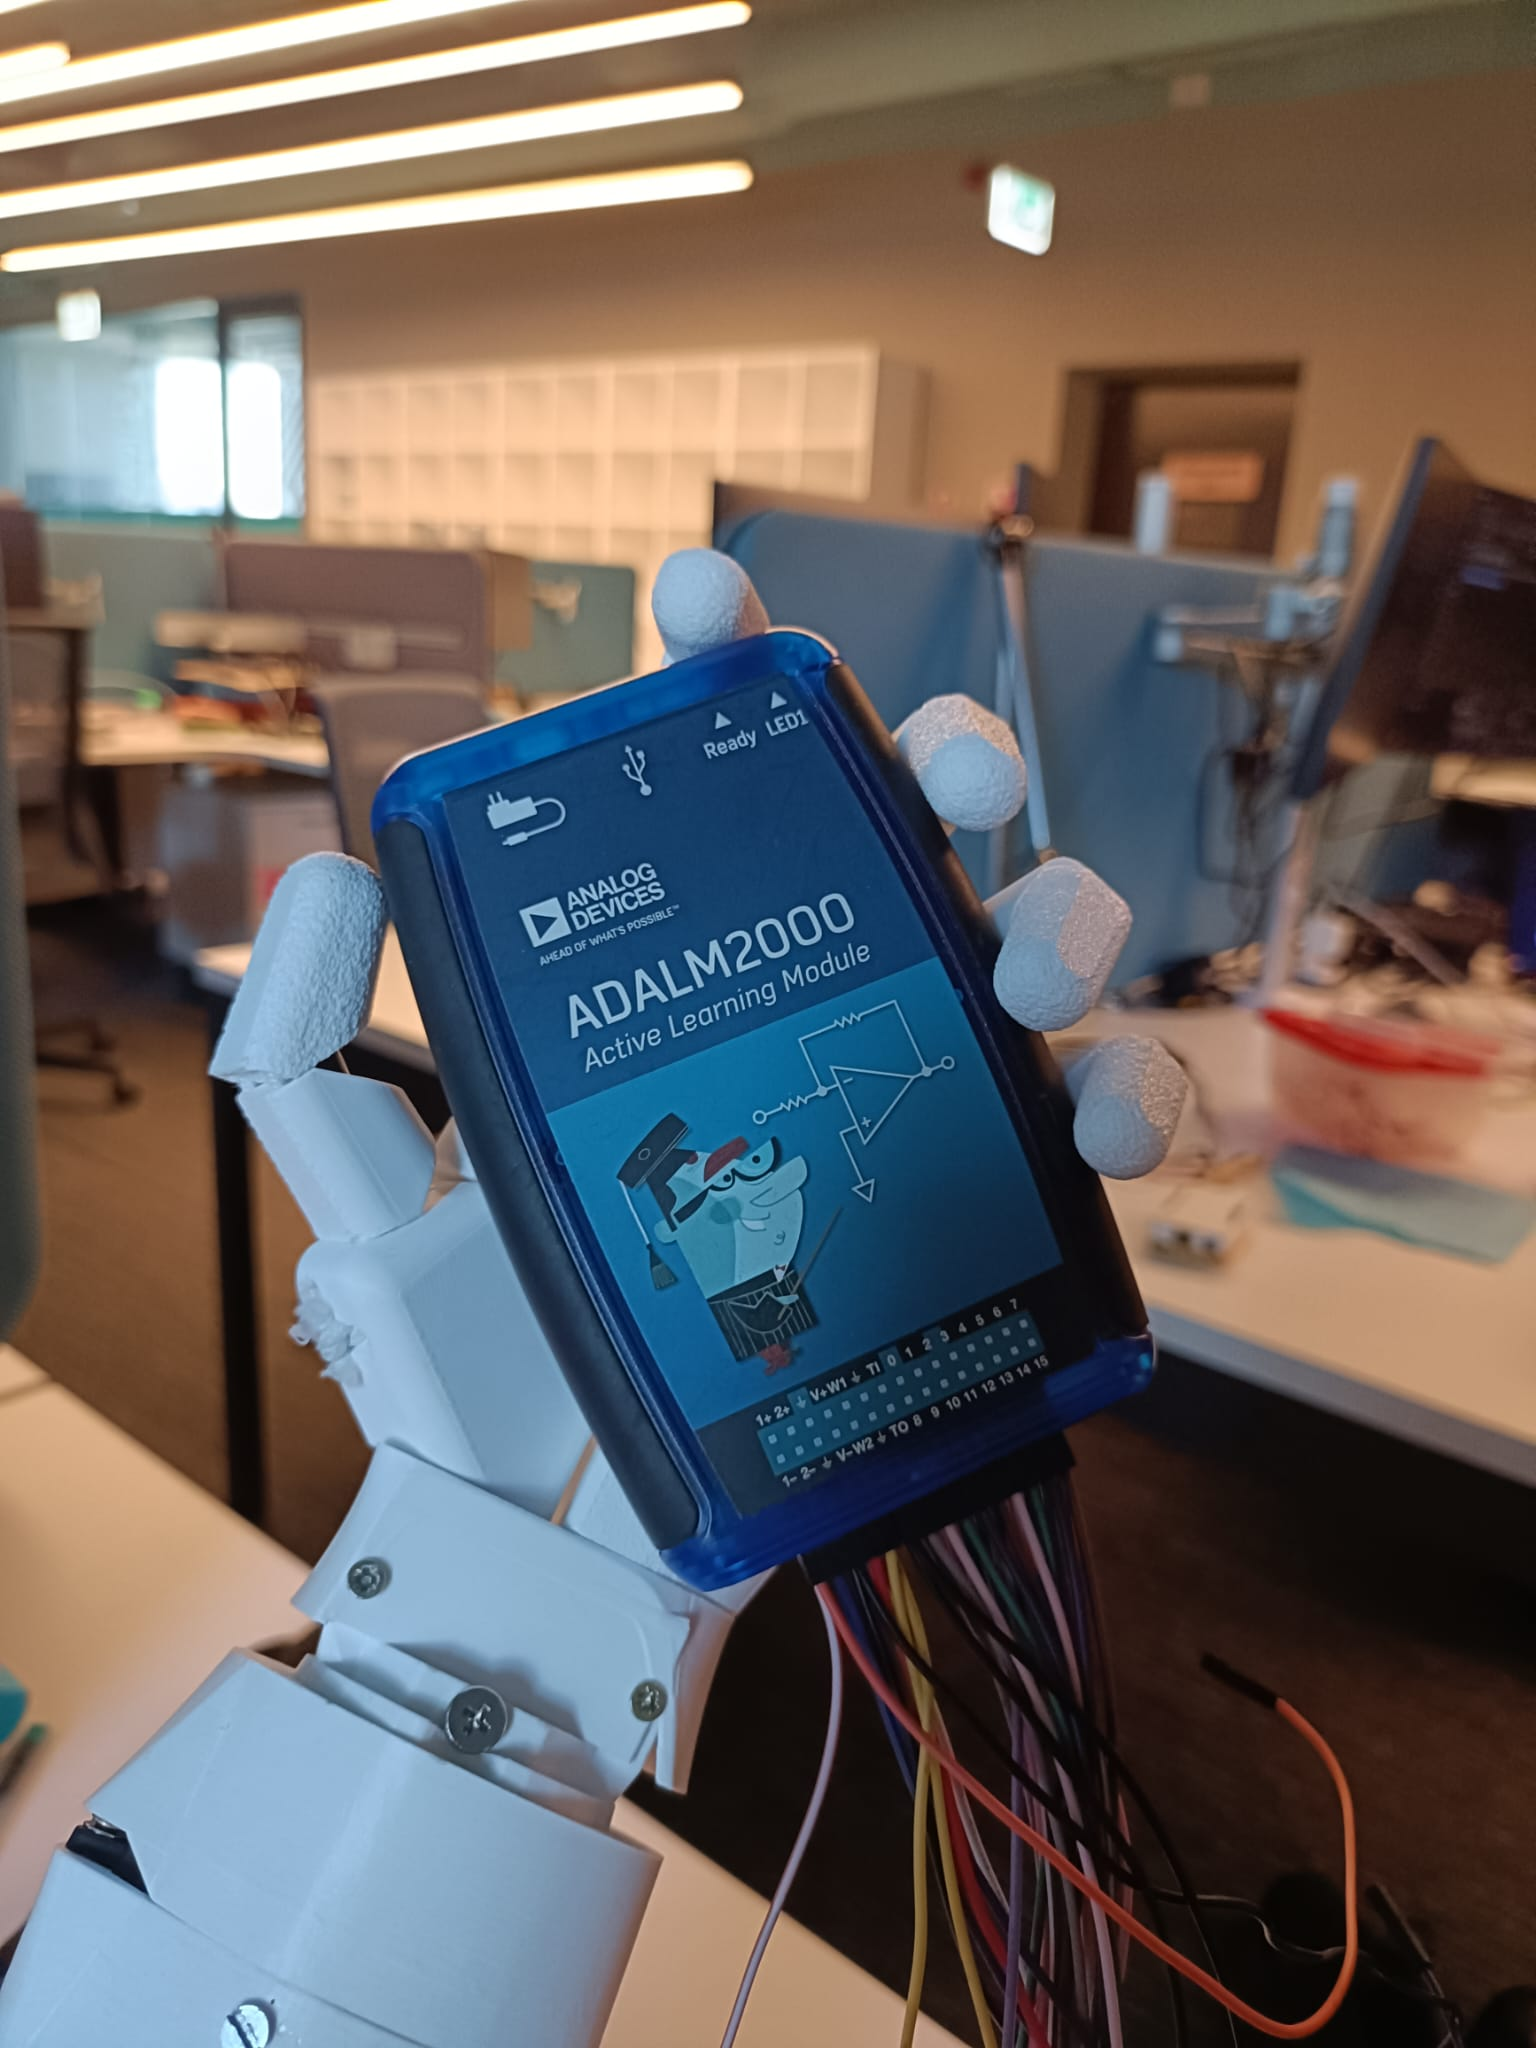
\includegraphics[width=0.42\textwidth]{figs/grip_adalm1.jpg}\hfill
	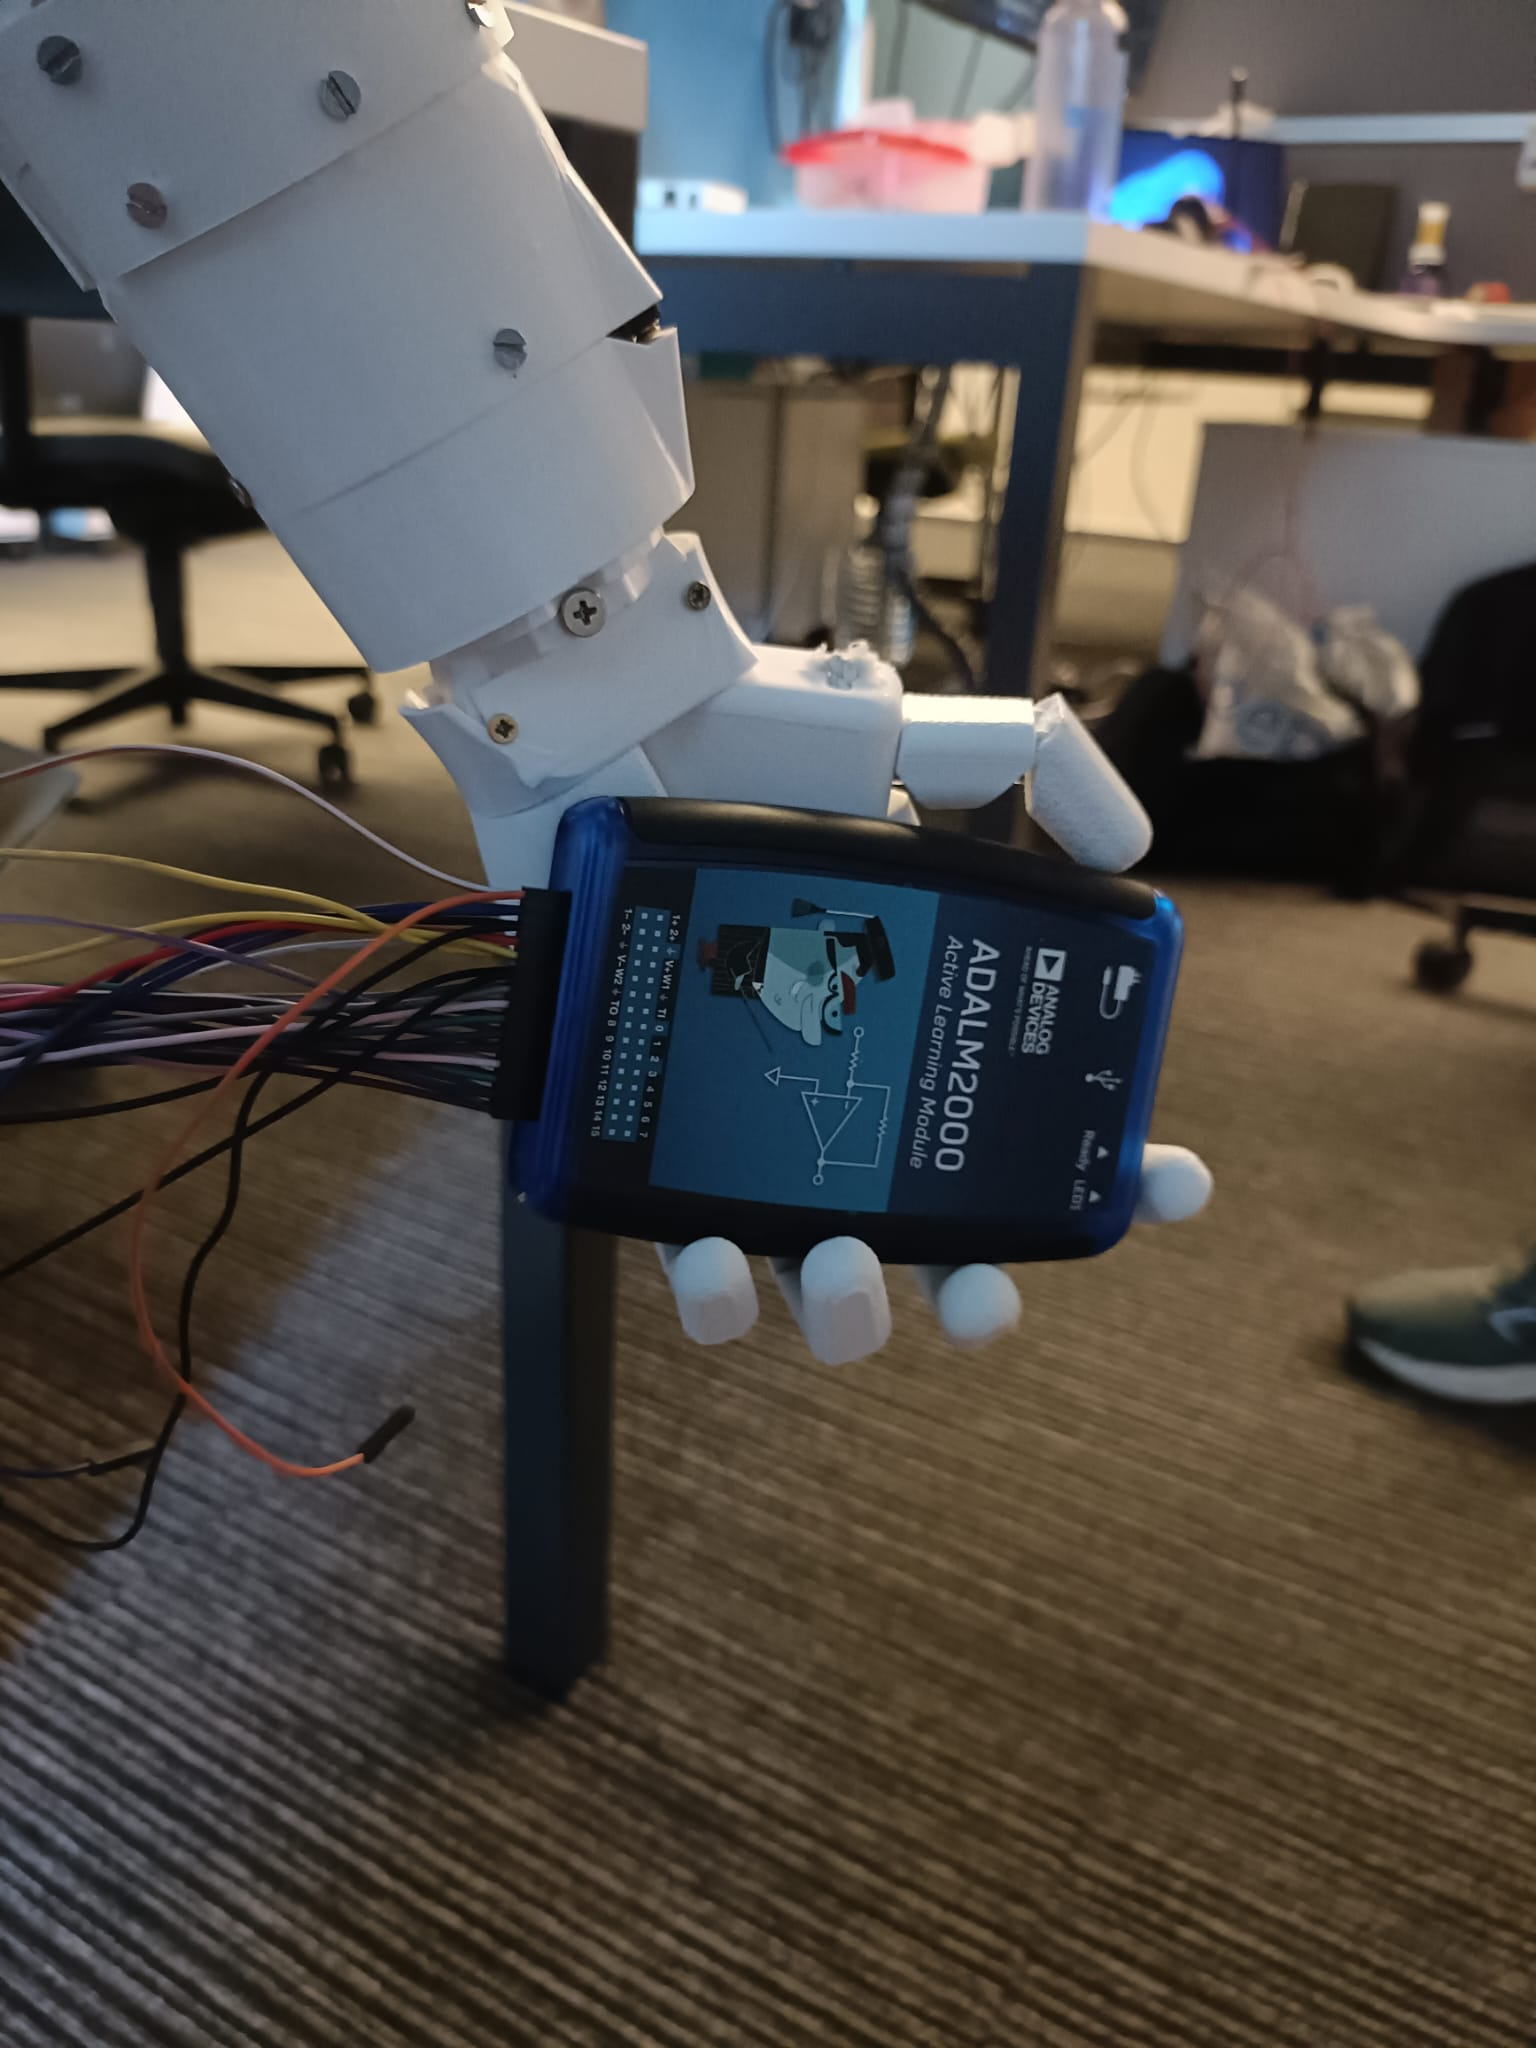
\includegraphics[width=0.42\textwidth]{figs/grip_adalm2.jpg}
	\caption{Mâna robotică prinzând un modul electronic, văzută din două unghiuri.}
	\label{fig:grip-adalm}
\end{figure}

În Figura~\ref{fig:grip-mosor} este prezentată prinderea unui mosor de fir de pescuit,
un obiect cilindric. În ambele situații, degetele s-au adaptat formei obiectului, iar
prinderea a fost suficient de fermă pentru a-l susține fără să alunece.

\begin{figure}[t]
	\centering
	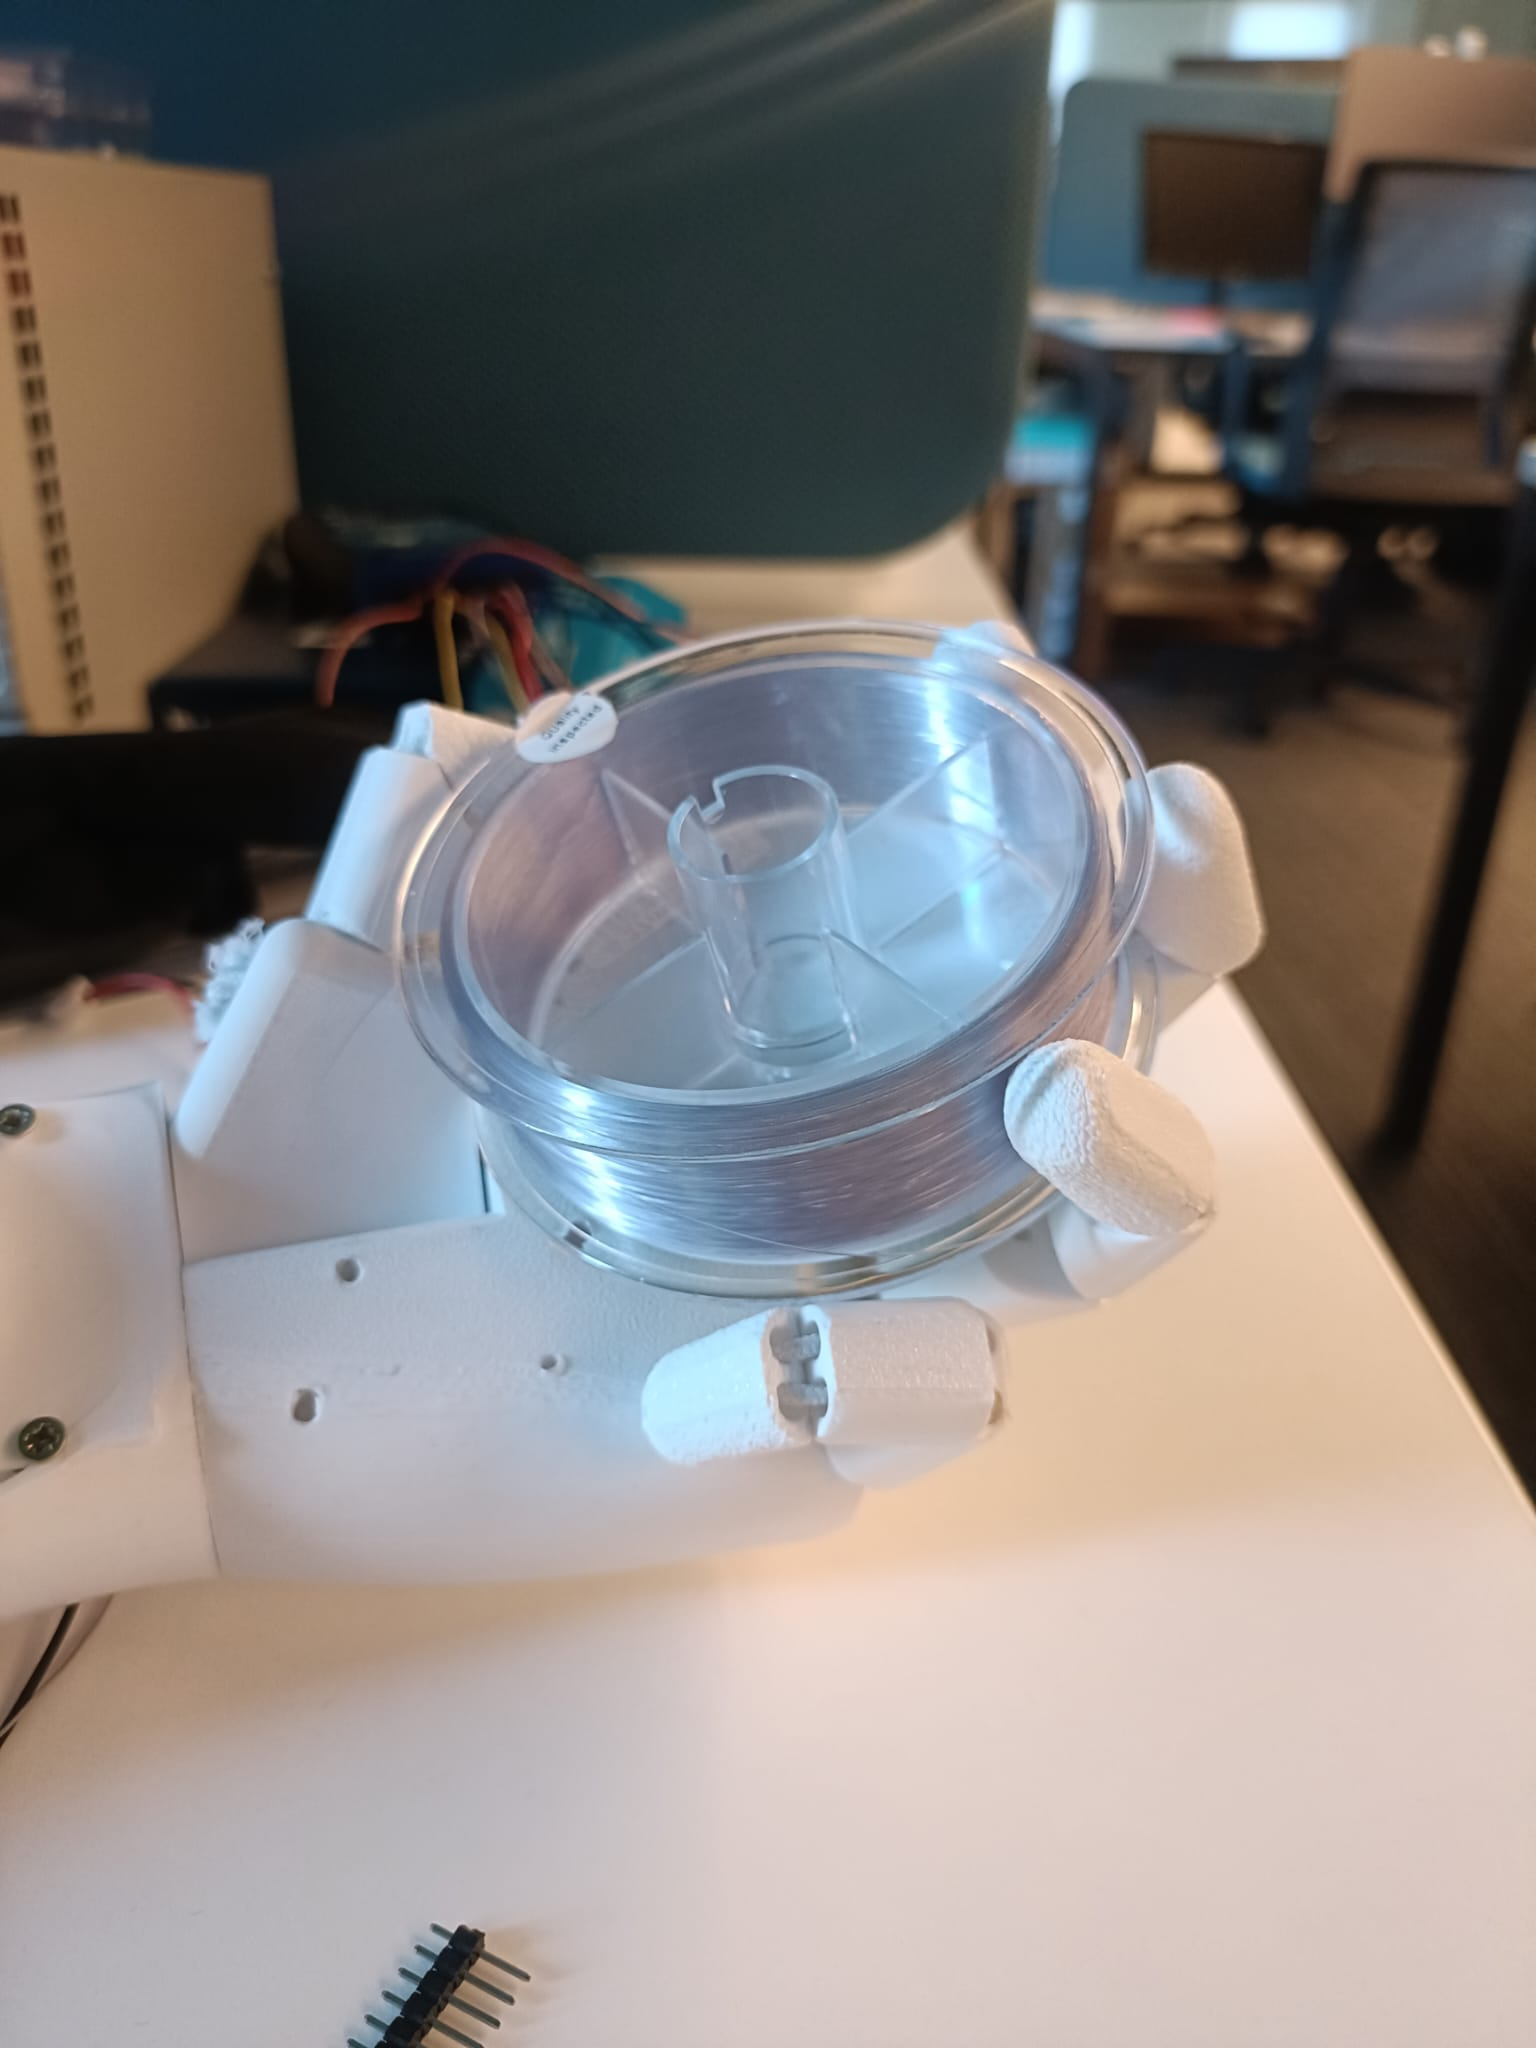
\includegraphics[width=0.48\textwidth]{figs/grip_mosor.jpg}
	\caption{Mâna robotică prinzând un mosor de fir de pescuit.}
	\label{fig:grip-mosor}
\end{figure}

Rezultatele testelor de prindere sunt sintetizate în Tabelul~\ref{tab:grip}. S-a observat
că prinderea este fermă pentru obiectele cu suprafețe care oferă aderență, dar mai puțin
sigură pentru obiectele netede din plastic lucios, precum sticlele, care tind să alunece
printre degete. Acest comportament este de așteptat, deoarece degetele nu dispun de un
material antiderapant la vârfuri, iar îmbunătățirea aderenței reprezintă o direcție
posibilă de dezvoltare ulterioară.

\begin{table}[H]
\centering
\caption{Rezultatele testelor de prindere pe diferite obiecte.}
\label{tab:grip}
\begin{tabular}{l l c}
\toprule
\textbf{Obiect} & \textbf{Formă} & \textbf{Prindere fermă} \\
\midrule
Modul electronic & plană, cu muchii & da \\
Mosor de fir de pescuit & cilindrică & da \\
Sticlă din plastic & cilindrică, netedă & alunecă \\
\bottomrule
\end{tabular}
\end{table}

\section{Analiza rezultatelor}
\label{sec:testare-analiza}

Testele efectuate confirmă că sistemul își îndeplinește scopul propus. Partea digitală
funcționează corect și stabil pe placa FPGA, respectând constrângerile temporale, iar
partea mecanică permite mâinii să reproducă mișcările comandate și să realizeze prize
funcționale asupra obiectelor uzuale. Abordarea de testare pe niveluri s-a dovedit
eficientă, integrarea finală decurgând fără probleme majore tocmai datorită validării
prealabile a fiecărui subsistem.

Ca o ultimă verificare, sistemul a fost testat și împreună cu partea de viziune dezvoltată
de colegul meu, în care mâna reproduce în timp real gesturile capturate de la o cameră.
Deși integrarea completă a celor două componente depășește obiectivul acestei lucrări,
această probă a demonstrat că lanțul întreg, de la captura video până la mișcarea mâinii,
poate funcționa unitar, validând conceptul de teleoperare care a stat la baza proiectului.
